\documentclass{article}
\usepackage{graphicx}
\usepackage{subfig}
\begin{document}

So Ivan had predicted that we could extract $\textbf{Var}(\tilde{h}^{KPZ}(0, s))$ from the relation:

\begin{equation}
\textbf{Var}(\tilde{h}^{KPZ}(0, s)) \approx \frac{s}{\log(N)}\textbf{var}(Q_{B}(N, \frac{\log(N)^{2}}{s}))
\end{equation}

where $s=\frac{\log(N)}{t}$ and $Q_{B}(N, t)$ is the position of the Nth quantile at time t. A graph of $\textbf{Var}(\tilde{h}^{KPZ}(0, s))$ is shown below as the blue triangles. I think the key feature is that it's monotonically decreasing and as $t \rightarrow \infty$ it approaches a value between 0.5 and 1.

\begin{figure}[h]
\centering
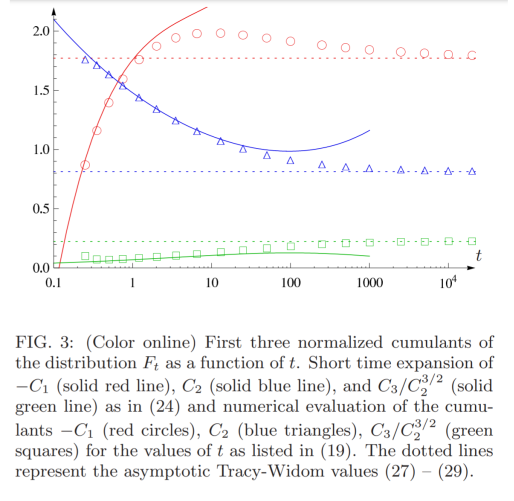
\includegraphics[width=8cm]{KPZGraph}
\caption{Variance of $\tilde{h}^{KPZ}$ is the blue triangles.}
\end{figure}

We'd like to plot the right side of Equation 1 as a function of $s$; however, the issue is we have only recorded $\textbf{var}(Q_{B}(N, t)$ as a function of time so we need to transform this to match Equation 1. So we'd like to plot:

\begin{equation}
\frac{s}{\log(N)}\textbf{var}(Q_{B}(N, \frac{\log(N)^{2}}{s}))  \textrm{ vs. }  s
\end{equation}

If we plug in $s$ we get

\begin{equation}
\frac{t}{\log(N)^{3}}\textbf{var}(Q_{B}(N, \frac{\log(N)^{4}}{t}))  \textrm{ vs. }  \frac{t}{\log(N)^{2}}
\end{equation}

My thought was to transform this so that on the LHS we have $\textbf{var}(Q_{B}(N, t'))$. I began by substituting in $t' = \frac{\log(N)^{4}}{t}$ so we get

\begin{equation}
\frac{\log(N)}{t'}\textbf{var}(Q_{B}(N, t'))  \textrm{ vs. }  \frac{\log(N)^{2}}{t'}
\end{equation}

Now my assumption was that plotting Equation 4 would be the same as Equation 1 which should give us the points in Figure 1. When I did this I got the figure below which doesn't look like the curve in Figure 1 at any times.

\begin{figure}[h]
\centering
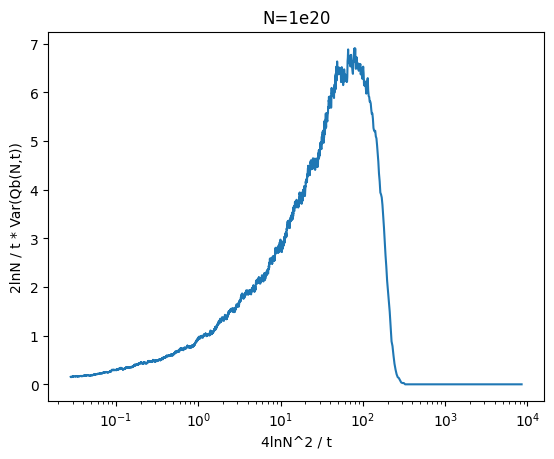
\includegraphics[width=8cm]{KPZVar1e20}
\caption{Calculated curve for $\tilde{h}^{KPZ}(0, s)$}
\end{figure}

The figure was generated using the PDF for ~1000 systems out to t=300,000 and for the 1e20 quantile.

\end{document}
